\documentclass{article}
\usepackage{graphicx} % Required for inserting images
\usepackage{float}
\usepackage{hyperref}
\usepackage{geometry}
\geometry{margin=2cm}

\title{ElecSoc Soldering Practice Card}
\author{JayceDesign}
\date{August 2024}

\begin{document}

\maketitle

\section{Introduction}
The practice card is an oscillating circuit with a 555 timer. It blinks 2 sets of LEDs. The oscillating period is controlled with an RC circuit.

\section{Assembling the board}
The board has 2 sets of components. Required and optional components. The required components are the minimum components needed to assembled to have a working card. The optional components are for soldering practice and to change the oscillator circuit. The required components are marked with an asterisk in the board.\\
To assemble the card, start with the bigger packages first. There are 4 different packages: 1206, 0805, 0603 and 0402. The bigger the number, the bigger the component, and easier to solder it will be. Start with the practice components first. Assemble first the optional 1206 resistors, then the 0805 LEDs. Then, move on to the practice network on the bottom left of the card. Then, start placing on the required components, from the largest package to the smallest. Lastly, solder on the 555 timer and the pin headers on the left.
\begin{figure} [H]
    \centering
    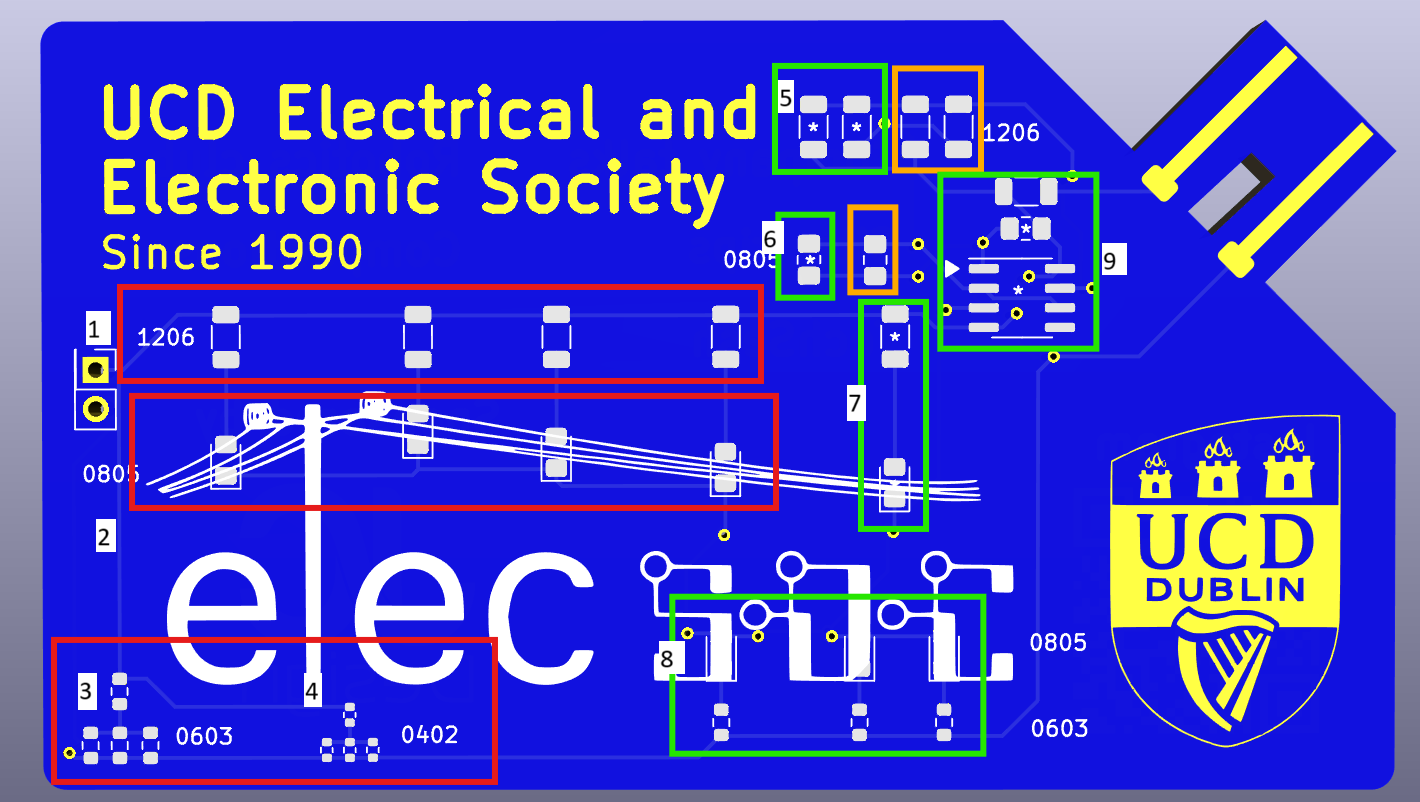
\includegraphics[width=0.6\linewidth]{Practice board marked.png}
    \caption{The order of soldering is indicated above.}
    \label{fig:enter-label}
\end{figure}
In red, the practice components. Green, components to assembled once comfortable with the process. Orange, extra components for tuning oscillating circuit. You don't need to solder all optional components, only as many as you need to feel comfortable with the soldering process.
\section{Testing}
If properly assembled, when the card is powered, the LEDs will blink with a period of 1.5s. The practice network is a voltage divider. The voltage drop at the lower resistors should be 1.25V. If you add the 5$\Omega$ resistor on the top right, you can slot the card in a USB port.\\
You can add the optional resistors for the oscillator circuit. This will reduce the period to about 0.8s. Adding only the extra capacitor will increase the period to 3.3s.

\end{document}
